\def\problemset#1#2#3{
\noindent\rule{16.5cm}{1pt}
\begin{center}
  \parbox{16.5cm}{\bf
    STAT 598Z Homework 4 \\
    Instructor: Prof. S V N Vishwanathan \hfill Jiajie Huang\\
    Due March 19th, 2013 \hfill huang147@purdue.edu
    }
\end{center}
\noindent\rule{16.5cm}{0.5pt}
}

\newcommand{\lb}[1]{\left \lfloor #1 \right \rfloor}
\newcommand{\bmat}[1]{\begin{bmatrix} #1 \end{bmatrix}}
\documentclass[fleqn, 11pt]{article}
\usepackage{fullpage}
\usepackage{hyperref}
\usepackage{ulem}
\usepackage{amsmath}
\usepackage{algorithm}
%\usepackage{algorithmic}
\usepackage{algpseudocode}
\setlength{\parindent}{0in}
\usepackage{graphics}
\usepackage{graphicx}
\usepackage{mathtools}


\begin{document}

\problemset{3}{Problem Set 2}{\today}


\section*{Problem 1}
This problem can be solved by two different methods: either accept-reject sampling or coordinate transformation (similar to the orthogonal and polar coordinate transformation that learned in class). 
\begin{itemize}
\item Accept-reject Sampling. This method is very straightforward. Just simply generate $x$ and $y$ from $uniform(-1,1)$, then look at the range of $x$ and $y$ together, only the $(x,y)$ pairs that fall into the shaded square are accepted. The efficiency of this method is about $0.5$. 

\item Coordinate transform. Consider a square bounded by four lines: 
\[x=-\sqrt{2}/2\]
\[x=\sqrt{2}/2\]
\[y=-\sqrt{2}/2\]
\[y=\sqrt{2}/2\]

If we rotate the square and its coordinate counter clockwise by $\theta=45^{\circ}$, we get the desired shaded square in this problem. We can easily sample $(x,y)$ from the original square, and then use coordinate transformation to get $(x',y')$ in our desired rotated square. The equation for getting an orthogonal coordinate transformation by an angle (counter clockwise) of $\theta$ is 
\[
\begin{cases}
x'=x\cos\theta+y\sin\theta=\sqrt{2}/2*x+\sqrt{2}/2*y \\
y'=-x\sin\theta+y\cos\theta=-\sqrt{2}/2*x+\sqrt{2}/2*y
\end{cases}
\]
\end{itemize}  

See Figure \ref{two} for a comparison of these two methods below.  \\\\

\begin{figure}[htb]
\centering
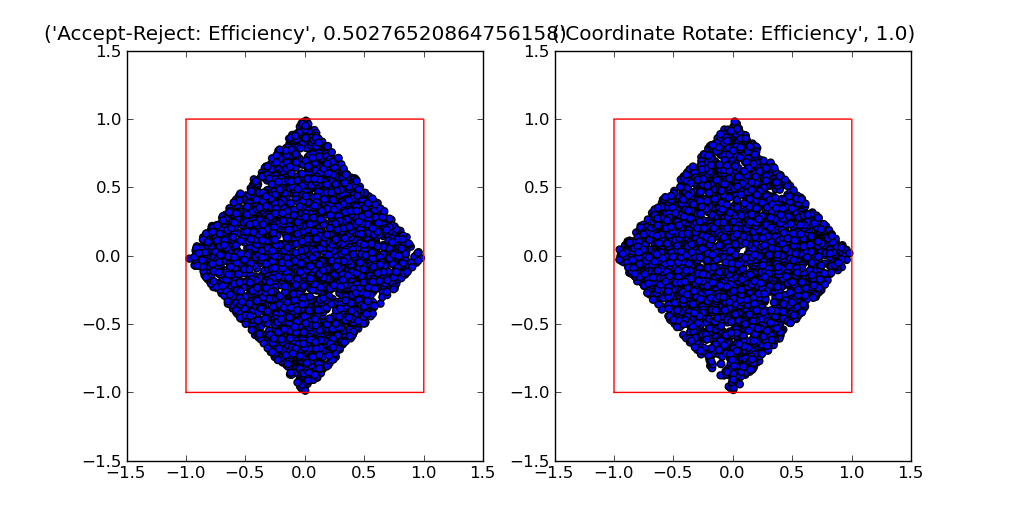
\includegraphics[width=18cm]{p1.png}
\caption{Comparison of Accept-Reject Sampling, and Coordinate Rotation }
\label{two}
\end{figure}




\section*{Problem 2}
Since $X\sim Beta(1,\beta)$, we have the pdf of $X$
\[
f_X(x)=\frac{1}{B(1,\beta)}x^{1-1}(1-x)^{\beta-1}=\frac{1}{\int_0^1 (1-t)^{\beta-1}dt}(1-x)^{\beta-1}=\beta(1-x)^{\beta-1} \\ (0\leq x \leq 1)
\]

and $Y\sim X^{\frac{1}{\gamma}}$, we have the pdf of $Y$ from transformation of $X$
\[
f_Y(y)=f_X(g^{-1}(y))|\frac{dx}{dy}|=\beta(1-y^{\gamma})^{\beta-1}\gamma y^{\gamma-1}=\gamma\beta y^{\gamma-1}(1-y^{\gamma})^{\beta-1}
\]
From integration we have the cdf of $Y$
\[
F_Y(y)
=\int_0^y f_Y(t)dt 
= \int_0^y \gamma\beta t^{\gamma}(1-t^{\gamma})^{\beta-1}dt
=1-(1-y^{\gamma})^{\beta}
\]
From inverse transformation, we have 
\[
F_Y^{-1}(u)=[1-(1-u)^{\frac{1}{\beta}}]^{\frac{1}{\gamma}}
\]
Which means we only need to draw samples from $u\sim uniform(0,1)$, and then transform it into $F_Y^{-1}(u)$ to get the sample of $Y$. See my code in the attached pages. Figure \ref{beta} is showing the plot of histogram versus the function itself. 

\begin{figure}[htb]
\centering
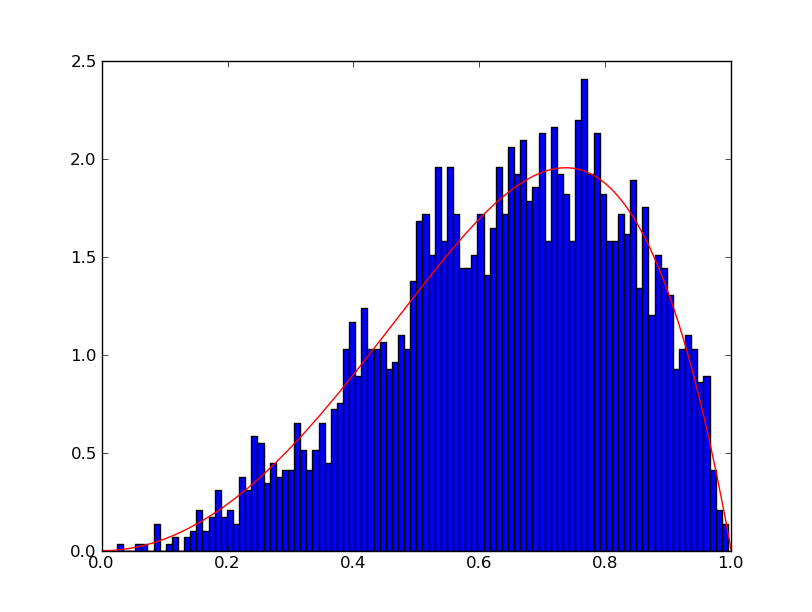
\includegraphics[width=18cm]{p2.png}
\caption{Plot of histogram and function of Y}
\label{beta}
\end{figure}


\end{document}